\documentclass{article}
\usepackage{graphicx}
\usepackage{subcaption}

\title{Report 9: Gather Pattern - Histogram Equalization}
\author{Nam Le}
\date{\today}

\begin{document}

\maketitle

\section{Methodology}
I implemented the Histogram Equalization algorithm based on Slides 21--30 using the Gather pattern:
\begin{enumerate}
    \item \textbf{Grayscale Conversion (Map)}: Converted the input RGB image into a 2D grayscale image on GPU.
    \item \textbf{Histogram Calculation (LW 9a)}: Computed the 256-bin intensity histogram on CPU as instructed in Slide 24.
    \item \textbf{CDF \& LUT Construction}: Normalized the histogram to probability density $p_j = \frac{histo_j}{N}$, calculated the Cumulative Distribution Function $c_i = \sum_{j=0}^{i} p_j$ sequentially (Slide 30), and generated a Look-Up Table (LUT) scaled to $[0..255]$.
    \item \textbf{Histogram Equalization (LW 9b - Gather)}: Applied the LUT to remap pixel intensities on GPU via \texttt{apply\_equalization\_gpu}, where each thread gathers its new intensity from \texttt{lut[old\_val]}.
\end{enumerate}

\section{Experimental Results}
The pipeline was evaluated across three 2D block size configurations: $(8, 8)$, $(16, 16)$, and $(32, 32)$.

\begin{figure}[h]
    \centering
    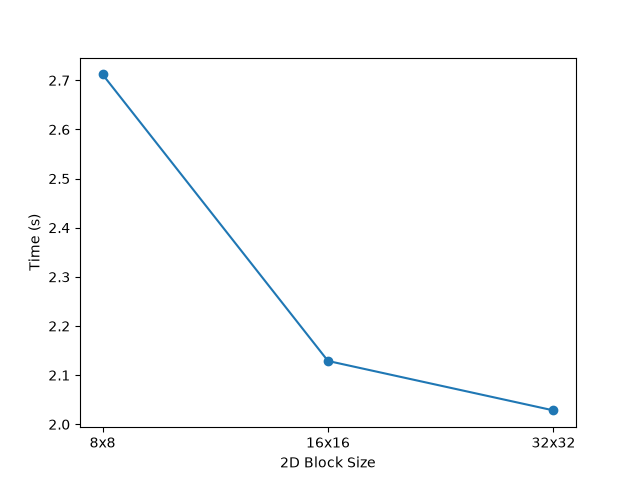
\includegraphics[width=0.65\textwidth]{gather_block_size_vs_time.png}
    \caption{2D Block Size vs Execution Time for Labwork 9}
\end{figure}

\begin{figure}[h]
    \centering
    \begin{subfigure}[b]{0.45\textwidth}
        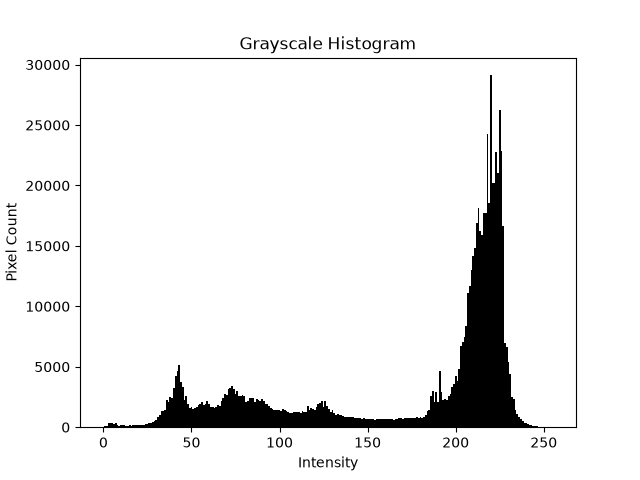
\includegraphics[width=\textwidth]{histogram.png}
        \caption{Grayscale Intensity Histogram}
    \end{subfigure}
    \hfill
    \begin{subfigure}[b]{0.45\textwidth}
        
\includegraphics[width=\textwidth]{equalized.jpg}
        \caption{Equalized Image Output}
    \end{subfigure}
    \caption{Intensity Histogram and Equalized Result}
\end{figure}

\section{Discussion}
\begin{itemize}
    \item The output image demonstrates a significant improvement in global contrast, revealing subtle details in dark and bright areas.
    \item Execution time steadily reduced from $2.71$ seconds at $(8, 8)$ to $2.13$ seconds at $(16, 16)$ and $2.03$ seconds at $(32, 32)$.
    \item Larger 2D block sizes improved thread occupancy and latency hiding during GPU memory access.
\end{itemize}

\end{document}
